\section{Funzionamento generale}
Le Convolutional Neural Networks~\cite{reti}, o reti di convoluzione, sono reti specializzate 
nell'elaborazione di dati che hanno la forma di vettori multipli con una topologia 
nota a forma di griglia. Esse nascono nel 1990 dalla ricerca di Yann LeCun 
insieme al suo team basandosi sul funzionamento della corteccia visiva del
 cervello umano. Grazie alle ottime prestazioni che si sono riuscite a ricavare 
 soprattutto in ambito del riconoscimento di immagini, ancora oggi le
CNN sono considerate lo “stato dell’arte” per quanto riguarda riconoscimento di
 pattern ed immagini.  \\
Un’immagine può essere vista come una griglia di due dimensioni di pixel 
contenente i tre valori di intensità per i tre canali del colore (RGB). L'immagine digitale letta dalla libreria OpenCV può essere vista come una matrice tridimensionale di valori compresi tra 0 e 255.\\
Il nome rete di convoluzione è dato appunto dal fatto che durante il suo 
funzionamento esegue un’operazione matematica chiamata convoluzione. \\
Un aspetto chiave di ogni algoritmo di Machine Learning è quello di riuscire
 ad estrarre i tratti più importanti dai dati in ingresso. Le CNN sono 
 in grado di capire in maniera automatica i tratti più rilevanti e di apprenderne 
 i pattern~\cite{cnn}; per questo motivo di norma gli strati delle CNN vengono considerati 
 come dei blocchi per rilevare i tratti: i primi strati (quelli subito dopo lo
  strato di ingresso) sono considerati “low-level features extractors”, mentre
   gli ultimi strati (di solito completamente connessi come quelli delle Reti 
   Neurali non convolutive discusse all’inizio) sono considerati 
   “high-level features extractors”. \\
   A ciascuna immagine di addestramento vengono applicati dei filtri 
   a diverse risoluzioni e l’output di ciascuna immagine convoluta viene utilizzato 
   come input per il layer successivo. I filtri possono essere inizialmente feature 
   molto semplici, ad esempio la luminosità o i bordi (low level features), e diventare sempre più
    complessi fino a includere feature che definiscono in modo univoco l’oggetto (high level features).
   Le CNN elaborano delle \emph{mappe dei tratti} (o \emph{feture maps}) dove ogni elemento corrisponde
    a dei pixel nell’immagine originale. Per ottenere questo risultato è necessario
     effettuare appunto l’operazione di convoluzione.\\
    
\section{Architettura generale di una CNN}
\subsection{Convoluzione}
Una CNN usa la convoluzione al posto del generale prodotto matriciale in 
almeno uno dei suoi strati. 
La convoluzione è una operazione su due funzioni a valori reali; 
dette queste due funzioni \emph{x} e \emph{w}, il loro prodotto di convoluzione sarà
\[s(t) = \int x(a)w(t-a) da = (x * w) (t).\]
Nelle reti di convoluzione spesso la funzione \emph{x} si riferisce
 alla funzione di ingresso e la funzione \emph{w} al kernel, che può essere visto come una funzione
  di peso relativa ai dati di input. Più in generale, nelle applicazioni l’input 
  è un vettore multidimensionale dei dati e il kernel è un altro array 
  multidimensionale di parametri che vengono adattati dall’algoritmo di
   apprendimento in maniera appropriata. Per utilità pratiche conviene 
   definire nello specifico l’operazione di convoluzione discreta, 
   un prodotto di convoluzione che invece di essere implementato su un integrale
    esteso all’infinito è implementato su una sommatoria su un numero finito di 
    indici riferiti agli elementi dei vettori. Per esempio, avendo come input
     una immagine bidimensionale I, si potrà usare un kernel bidimensionale W tale che:
\[S(i, j) = ( I * W )(i, j) = \sum_{m}\sum_{n} I(m, n)W(i-m, j-n).\]
Spesso nelle implementazioni software si preferisce utilizzare una funzione che si basa su quella sopra,
 chiamata cross-correlation, che è la stessa della convoluzione ma con
  il kernel capovolto. 
  \[S(i, j) = ( I * W )(i, j) = \sum_{m}\sum_{n} I(i+m, j+n)W(m, n).\]
Sotto si può vedere una figura che mostra un esempio di feature che un filtro di convoluzione è in grado di estrarre (Figura 3.1).
     
\begin{figure}[H]
     \centering
     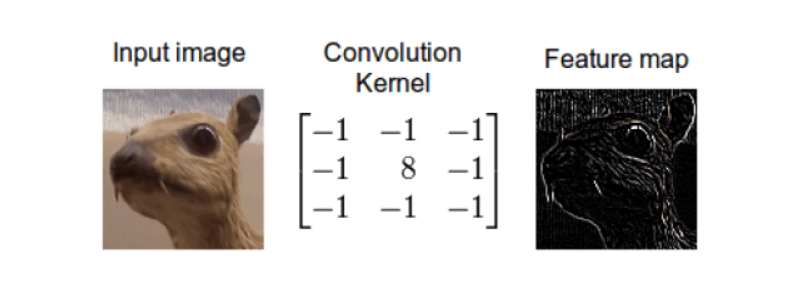
\includegraphics[width=0.8\textwidth]{Figures/feature map.PNG}
     \caption{\small{Questo kernel è in grado di identificare i bordi della sagoma dell'animale nell'immagine tramite una precisa disposizione dei valori dei pesi nella matrice stessa.~\cite{feature}}
     } % end caption
     \label{fi:dcalc}
   \end{figure}
   
Vi sono due concetti alla base del funzionamento delle CNN :\\
\begin{enumerate}
     \item \emph{Sparse Connectivity} (connessioni locali)~\cite{sparse}; l’idea è che, in un'immagine in cui i pixel sono spazialmente più vicini, questi siano
 più propensi a rappresentare
 qualcosa di correlato tra di essi. 
Per esempio, nell’analisi di una immagine di input che abbia centinaia o milioni di pixel 
siamo interessati a individuare feature significative o dettagli importanti molto piccoli
 rispetto alla dimensione totale dell’immagine, contenuti per esempio in una decina di pixel 
 come ordine di grandezza.
Gli strati tradizionali delle reti neurali usano il prodotto matriciale tra matrici di parametri
 che descrivono l’interazione tra ogni unità di input con ogni singolo output; questo significa
  che ogni unità di output interagisce con ogni unità di input.
   Le reti di convoluzione invece possono avere connessioni locali tra i neuroni che generano 
   interazioni sparse nella rete. Questa connessione locale può essere formalizzata impostando 
   il kernel più piccolo rispetto all'input. 
Dati m input e n output, un prodotto matriciale richiederebbe m·n parametri e l’algoritmo 
una complessità temporale O(mn) di elaborazione. Limitando il numero di connessioni per ogni 
output ad un numero k più piccolo di m sarebbero richiesti solo k ·n parametri e un tempo di 
elaborazione pari a O(k ·n). Il guadagno in efficienza diventa estremamente importante con k
 più piccoli di m di molti ordini di grandezza.\\
  Dunque l’idea della convoluzione è di preservare le relazioni spaziali tra i pixel. 
Ridurre il numero di connessioni regolarizza la rete e riduce il rischio di overfitting. 

\item \emph{Parameter-sharing}~\cite{max-pool} (parametri condivisi): l'idea di base è che gli stessi pesi
 vengano utilizzati per diversi gruppi di pixel dell’immagine principale.\\
In una rete tradizionale, ogni elemento della matrice dei pesi è usato esattamente
 una volta durante il calcolo di un output dello strato e poi non viene più riutilizzato. 
 Qui gli stessi pesi vengono utilizzati per diversi gruppi di pixel dell’immagine principale.
  Il valore di un peso applicato ad un input è collegato al valore di un peso applicato in 
  un altro punto della rete. In una CNN ogni kernel utilizzato è fatto in modo tale da essere 
  invariante alle traslazioni, quindi è usato in tutte le posizioni dell’input 
  (eccetto che per alcune particolari condizioni al contorno). 
  La rete apprende quindi solo da un determinato set di parametri invece che da tanti 
  set separati per ogni sezione dell’input, il che riduce significativamente 
  il numero di accessi in memoria.  Inoltre si sa che così come i neuroni della corteccia
   cerebrale sono designati a riconoscere feature locali dell’immagine (come angoli o bordi), 
   si utilizzano gli stessi kernel (o filtri) per differenti parti dell’immagine, 
   sempre con gli stessi pesi e valori di attivazione. 

\end{enumerate}
 I neuroni degli strati
  di convoluzione sono organizzati nelle cosiddette \emph{feature maps},
   nelle quali ogni unità è connessa ad una porzione locale della mappa allo strato 
   seguente attraverso un insieme di pesi. Ogni feature map corrisponde ad un determinato
    \emph{kernel} che ha il fine di ricercare una certa feature in determinati punti dell’immagine.  
Data la definizione di convoluzione discreta descritta sopra,
 dato un filtro di dimensione k x k, con dei pesi associati atti a ricercare una determinata feature,
  e chiamato \(\theta\) il valore del bias si fa traslare il filtro lungo l’immagine 
  di input e si fa una somma pesata e shiftata rispetto a \(\theta\) salvando il risultato 
  ottenuto nelle feature maps stesse, che
   saranno tante quanti sono il numero di filtri applicato allo strato di input.
         
   \begin{figure}[H]
     \centering
     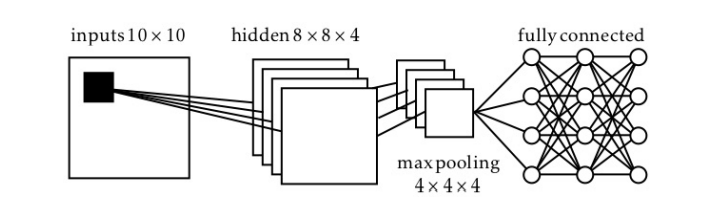
\includegraphics[width=0.8\textwidth]{Figures/cnn-schema.PNG}
     \caption{\small{Rappresentazione schematica di una CNN. Da sinistra verso destra: uno strato di input,
     le feature maps ottenute con la convoluzione, gli strati di max-pooling e infine la parte completamente connessa.~\cite{reti} % end small
     }
     } % end caption
     \label{fi:dcalc}
   \end{figure}
   
Il kernel viene shiftato ogni volta lungo la mappa dello strato precendente in orizzontale e  verticale
 di un valore s, detto \emph{stride}, che è un iperparametro molto importante nella
  fase di convoluzione.

La formula di convoluzione discreta scritta sopra è utilizzata per un array di due dimensioni. Per immagini
 colorate di solito si hanno 3 canali per colore, dunque in tale caso l’array 
 in input sarebbe tridimensionale. Si ottengono quindi array di dimensioni superiori a 2, 
 chiamati \emph{tensori}.
Tutti i neuroni di uno stesso strato convoluzionale hanno lo stesso valore del bias. 
 Il package software Tensorflow utilizzato nella fase sperimentale è atto a eseguire 
 efficientemente tutte le operazioni con i tensori. 
 \begin{figure}[H]
     \centering
     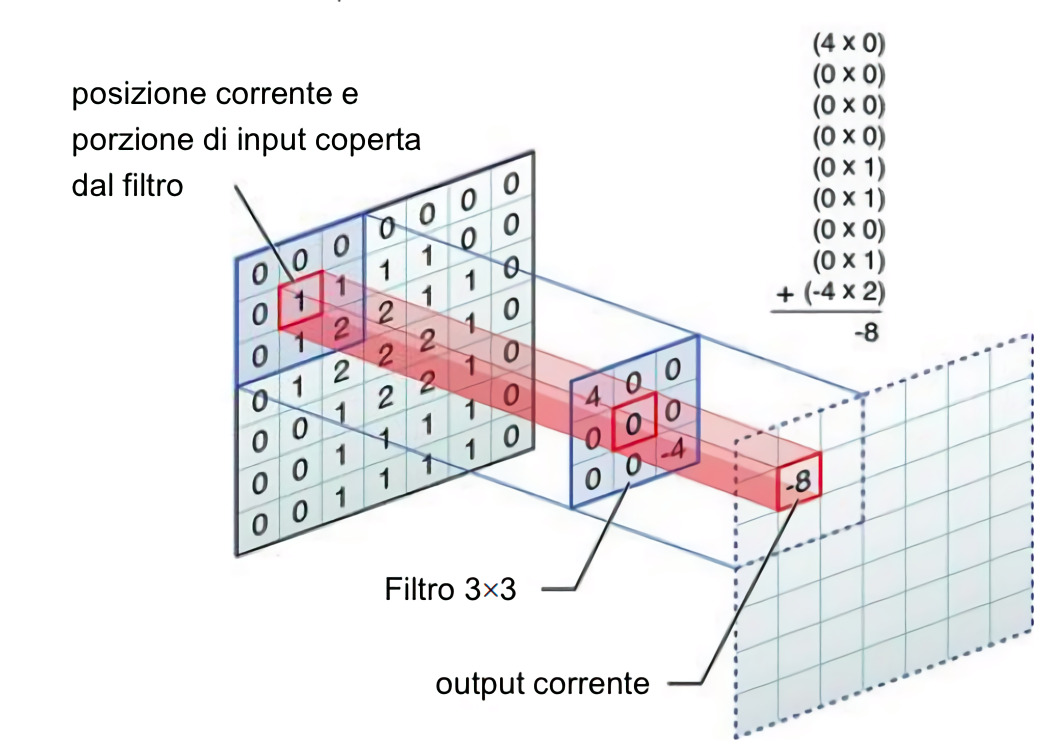
\includegraphics[width=0.8\textwidth]{Figures/convoluzione.jpg}
     \caption{\small{
          Schema di come avviene la convoluzione.~\cite{cnn}
     }
     } % end caption
     \label{fi:dcalc}
   \end{figure}
\subsection{Padding}
Se si accoppiano più strati di convoluzione l’uno dopo l’altro, a mano a mano 
che ci si muove verso destra il numero di neuroni decresce molto velocemente. 
E’ per questo che è necessario il padding, che permette di aggiungere righe o
 colonne di peso pari a 0, e che permettono l’utilizzo di filtri non troppo piccoli 
 senza dare problemi con le dimensioni in uscita. Esistono 3 tipi di padding ma quello utilizzato
  di più nell’implementazione di una CNN è il \emph{same padding}, il quale fa in modo di
   preservare le dimensioni dell’input originale.\\
   \begin{figure}[H]
     \centering
     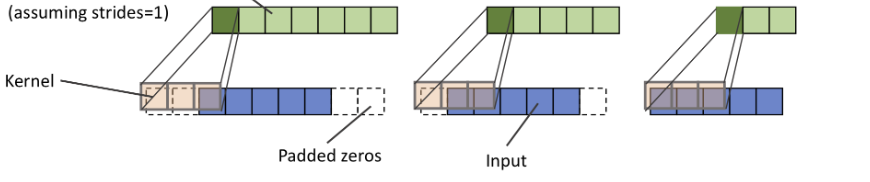
\includegraphics[width=0.8\textwidth]{Figures/padding.PNG}
     \caption{\small{
          Schema dei vari tipi di padding. A sinistra il padding di tipo \emph{full}, al centro quello di tipo \emph{same}, a destra il padding \emph{valid}~\cite{tesi}
     }
     } % end caption
     \label{fi:dcalc}
   \end{figure}
    Il sistema si calcola automaticamente il valore p di padding da adottare affinchè ciò 
    possa essere rispettato. 
La dimensione della feature map risultato di una convoluzione è data da:
$$ o = \frac{(n + 2p - m)}{s} + 1 $$ 
dove:
\begin{itemize}
     \item \emph{n} è la dimensione del vettore di ingresso (se è un’immagine si fa 
sempre in modo di renderla quadrata \emph{n} x \emph{n});
\item \emph{p}, come visto in precedenza è il valore di padding;
\item \emph{m} è la dimensione del filtro;
\item \emph{s} è lo stride.
\end{itemize}
Da qui è semplice ricavare \emph{p} per il same padding e/o \emph{s} per avere \emph{o} del valore desiderato.

\subsection{Funzioni di attivazione}
Come succede nelle reti neurali artificiali dense, anche nelle convoluzionali 
è necessario che, una volta fatta la convoluzione e generate le feature maps, i 
neuroni vengano passati attraverso una funzione di attivazione. 
Quella più utilizzata negli strati nascosti dei modelli nelle prove sperimentali è la ReLu
 (Rectified Linear Unit). Con questa le feature maps sono passate attraverso una
  funzione che ritorna zero se il valore in input è inferiore a 0, mentre ritorna il valore
   dell’input stesso se questo è maggiore di zero. \\
   Ciò è utile in quanto lo scopo di una CNN è quello di incrementare sempre di più la non
    linearità del dataset. Quando si guarda ad un immagine in effetti si nota come essa
     contenga molte zone non lineari come bordi, angoli, transizioni di colore… \\
     Lo scopo è quello di eliminare i pixel neri così da mantenere solo i grigi e i bianchi 
     rendendo la color transition più bruta ma più efficace al fine di identificare feature.\\
       La ReLu permette dunque di non attivare tutti i neuroni allo stesso momento, riducendo 
       il costo del processo di backpropagation necessario ad una corretta determinazione
        dei pesi durante il processo di training della rete, che è sicuramente più veloce
         se si procede in questo modo.
La convergenza della rete viene velocizzata di circa 6 volte di più rispetto
 a utilizzare una funzione di attivazione come la sigmoide o la tangente iperbolica.\\
 La ReLu verrà utilizzata anche perchè risolve in parte il problema della \emph{scomparsa del gradiente}~\cite{grad},
  uno dei 
 principali problemi del deep learning. Durante la fase di backpropagation i pesi degli strati in
  prossimità dell’input restano costanti o si aggiornano molto lentamente al contrario di quanto 
  accade per gli strati vicini all’output. Questo può provocare un rallentamento della rete ed è dovuto 
  alle funzioni di attivazione. Funzioni di attivazione come la sigmoide infatti sono funzioni a codominio
   limitato e hanno una derivata
    che presenta una regione di significatività (ovvero la regione del dominio dove la funzione derivata assume
     i valori più significativi) piuttosto piccola, oltre la quale il valore della derivata stessa
     è prossimo allo 0. Per la regola della catena nella fase di backpropagation è necessario 
     andare a fare un
      prodotto di derivate che è pari al numero di strati della rete neurale, come detto nella sezione 2.3.
       A mano a mano che però si torna 
      indietro dall’output verso l’input però, moltiplicando cifre molto 
      vicine allo zero tra di loro si
       ottengono valori di aggiornamento dei pesi infinitesimi che comportano l'impossibilità 
       per la rete di apprendere bene, soprattutto quando si vanno ad utilizzare reti 
       molto profonde, e quindi quelle tipiche del DL.


\subsection{Strati di subsampling: Pooling Layers}~\cite{cnn2}
Mentre il ruolo dello strato di convoluzione è quello di trovare congiunzioni locali tra feature
dello strato precedente, il ruolo dello strato di pooling è quello di fondere
 semanticamente feature simili in uno solo riducendo la dimensione dei dati.
Questo strato di solito è applicato subito dopo quello di convoluzione perchè lavora sull’output
 processato da questo strato e riprende il concetto di sparse connectivity.\\
  Un neurone di uno strato di pooling prende gli input di diverse feature maps
   vicine tra loro e li riduce ad un singolo output. 
Esistono due tipi di subsampling layers (strati di sottocampionamento) di questo tipo:\\
\begin{enumerate}
     \item \emph{Max Pooling}: le unità di questo strato calcolano il massimo di una porzione locale (definita a seconda della dimensione stabilita dal codice, ad esempio porzioni 2x2) in una mappa di feature. Allora una funzione di pooling sostituisce l’output di una rete ad una certa locazione con un risultato che riassume quelli ottenuti dagli output vicini, riducendo la dimensione della rappresentazione e focalizzando l’analisi solo sui punti salienti dell’oggetto analizzato. 
\item \emph{Mean Pooling}: in questo caso ogni neurone prende il valore medio dei valori 
della porzione di input. 
\end{enumerate}
In sintesi, un livello di pooling esegue un’aggregazione delle informazioni nel volume di input, 
generando feature maps di dimensione inferiore, conferendo invarianza rispetto 
a semplici trasformazioni dell’input, mantenendo al tempo stesso
le informazioni significative ai fini della discriminazione dei pattern contenuti in essi.\\
Se si ha una feature map di dimensione W x W x D, un kernel di pooling di dimensione F 
e un valore di stride pari a S, allora la dimensione dell’output sarà determinato dalla formula 
\[\frac{(W - F)}{S}+1\]
Il pooling funziona sull’idea di base per cui piccoli cambiamenti non cambieranno 
il risultato finale, perciò aggiunge robustezza ai dati. 
\begin{figure}[H]
     \centering
     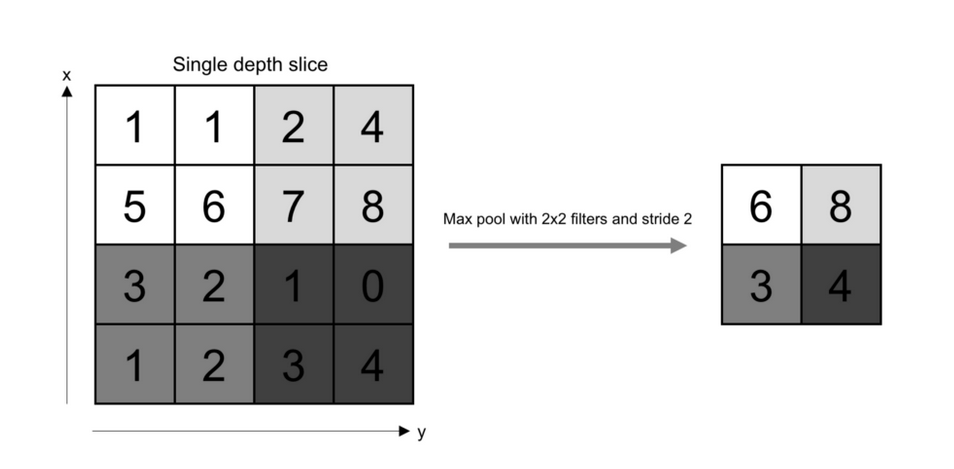
\includegraphics[width=0.8\textwidth]{Figures/pooling-ex.PNG}
     \caption{\small{
         Esempio di pooling tramite una pool 2x2. ~\cite{cnn2}
          }
     } % end caption
     \label{fi:dcalc}
   \end{figure}
\subsection{Fully connected layers}
Dopo gli strati di convoluzione/pooling si inseriscono uno o più strati di neuroni completamente connessi (Dense Layers), 
dopo aver compito un'operazione di Flattening di ogni feature map bidimensionale dello strato precedente.
I FC layers connettono tutti i neuroni del livello precedente con quelli del successivo al fine di stabilire 
le varie classi identificative visualizzate nei precedenti livelli secondo una determinata probabilità.
É grazie a questi strati che è possibile effettivamente poi ottenere un vettore in uscita
 che produca una stima probabilistica e che vada 
ad avere dimensione c x 1, dove c è il numero delle unità di classificazione. 

Ricapitolando, l’architettura di una CNN consiste generalmente di questi strati: 
\begin{itemize}
\item Input
\item Convoluzione 
\item Attivazione non lineare
\item Pooling 
\item Flattening
\item Dense layers
\item Output
\end{itemize}
Nella fase sperimentale del lavoro ne sono però stati utilizzati anche altri che saranno discussi in seguito.



